\documentclass[12pt,a4paper]{article}
\usepackage{ucs}
\usepackage{caption}
\usepackage[latin1,utf8x]{inputenc}
\usepackage{amsmath}
\usepackage{caption}
\captionsetup{font=small,labelfont=bf}
\usepackage[danish]{babel}
\usepackage[rmargin=3cm,tmargin=3.3cm]{geometry}
\usepackage{listings}
\usepackage{hyperref}
\setlength{\parindent}{0pt}
\setlength{\parskip}{1ex plus 0.5ex minus 0.2ex}
\usepackage{graphicx}
\usepackage{fixltx2e}

%insert links
\usepackage{hyperref}
\usepackage{fancyhdr,lastpage}	
\pagestyle{fancy}

%header
\lhead{ 
	Embedded Systems \\
	02131 \\ 
}
\chead{ 
}
\rhead{ 2 October, 2012 \\ \bigskip  }

%Footer
\lfoot{
	\rule{\textwidth}{0.1mm}\\
}

\cfoot{}
\rfoot{\ \\ \scriptsize{Side \thepage\ af \pageref{LastPage}}}

\begin{document}

%Forside
\begin{titlepage}
	\begin{center}
		\vspace*{13\baselineskip}
		\huge
		\bfseries
		Embedded Systems\\ 
		\ \\
		02131 \\[5\baselineskip]

		\normalfont
		\Large
		The ECG processor!\\	

		\small
		\vfill
	\end{center}	
	\begin{flushleft}
		Bastian Buch, s113432\\
	 	Jacob Gjerstruo, s113440\\
	\end{flushleft}
\end{titlepage}

\ \\
\section*{Abstract}
	The main task of this assignment was to develop a custom made processor which needs to be able to run the code for the ECG scanner, which was developed in the previous assignment. By using Gezel, we have created the basic modules for the processor, which would then need to be coupled together to create the actual processor, and furthermore, we have developed the instruction set for the processor, which is written in assembly code. Our conclusion is that we could quite easily connect the modules of the processor and thereafter start working on having this processor start on the instruction set, but unfortunately, we started too late in the project and ended up with a lack of time for doing this.
\thispagestyle{empty} 
\newpage

%Table of Contents
\tableofcontents
\thispagestyle{empty} 
\newpage

%Reset pagecount
\setcounter{page}{1}

%Alm. sider
\ \\
\section{Introduction}
For this part of the project, we were to continue our work for Medembed in designing and implementing a small embedded processor that can execute the QRS algorithm we developed. However, initially, we would first be required to implement only one filter - the Moving Window Integration filter - to demonstrate the capabilities of the processor - both in terms of size, speed and power consumption.\\
\\
We were tasked to make this implementation in the hardware description language called Gezel.\\
\section{Requirements}
For this assignment, we initially sat down and looked over the requirements, and in total, we found 4 functional requirements and one non-functional requirement. They are as follow: \\
\\
\textbf{ Functional requirements for the application:}
\begin{itemize}
	\item Creating the basic processor modules
	\item Creating the instruction set the processor must use
	\item Implementation of controller.
	\item An analysis of our implementation, including an analysis of the critical parts, runtime and memory requirements.
\end{itemize}
\textbf{Non-functional requirements for the application:}
\begin {itemize}
	\item The processor must be implemented in the Gezel language.
\end{itemize}

\section{Analysis}
 	In designing the actual ECG scanner, there are a few things that we had to consider.
\begin{enumerate}
	\item What are the basic modules of a processor?
	\item How should these modules be implemented?
	\item What instruction set should be used?
	\item How would the controller be implemented?
	\item How do you determine the critical parts?
\end{enumerate}

\subsection{Problem 1: The basic modules of a processor}
The first question we had to ask ourselves - what are the basic modules of a processor actually? This was a question that we needed to answer firstly, as without these basic modules, implementing the processor itself would be impossible.
\subsection{Problem 2: Implementation of the basic modules}
The second problem we considered was the question of how to actually implement these basic modules? Most seemed straight forward, but we encountered some issues in regards to the modules:\\
\begin{enumerate}
	\item In regards to the Arithmetic Logic Unit (ALU), how can the choices be implemented so the runtime is swift and the size is small?
	\item In regards to the memory, how can we read and write data, and furthermore, how should this data look?
	\item In regards to the Register, we had to figure out how we ensured that a registry always returned 0 no matter what.
\end{enumerate}
\subsection{Problem 3: The instruction set}
Designing the instruction set would have to be done manually, and this instruction set would need to be in assembly code, to ensure our processor can understand and interpret the instruction set correctly. Designing this instruction set could be done in multiple ways, and the biggest problem would be how to design this instruction set so it is as compact as possible, while ensuring that it is still compileable.

\subsection{Problem 4: Implementation of the controller}

\subsection{Problem 5: Critical parts}
When speaking of critical parts, there are three terms that needs to be discussed - size, speed and power. \\
The size of the processor is important because the larger it is, the more power-consuming it will be, and secondly, as the ECG scanner in itself cannot be that large, there is a maximum size the processor can have.\\
The speed is of course also important - the processor needs to be able to make a certain minimum number of calculations per second, in that the scanner itself, which will provide the processor with data, will bring 250 data points to be calculated on per second, and it is important that the processor is able to keep up with this stream of information. On the other hand, it is also important that the processor does not work too fast - having it consume lots of power to calculate, only to have it idle in-between data points would mean that energy is wasted, lowering the lifetime of the ECG scanner.\\
Finally, power consumption is important in that the more energy the processor consumes, the more often the battery on the scanner will need to be replaced or recharged - neither of which you want the costumer to bother with too often. The way to avoid this is either to reduce power consumption or to increase the battery size - the latter of which can only be done to a certain degree as the ECG scanner has a specific size.\\
\begin{enumerate}
\item How large would the processor be and can this size be reduced?
\item How fast is the processor, and how much idle time is there between data points?
\item What is the energy consumption and what can be done to reduce consumption?
\end{enumerate}

\section{Design}
When we were designing the basic modules, we very quickly decided to implement them in a testbench setting from the very beginning, as this made testing an easy and very comfortable thing. This setting simply consists of a test datapath as well as a Finite State Machine (FSM) to control the testbench and change the values of the registers, depending on the clock cycle.\\
Also, when we were designing the instruction set, we had to discuss whether we wanted to use a Div module or if we would make a loop that continually subtracted a set value until the value would be below 0. We decided to go with making a Div module - although this would mean we would need a more complicated module, it also means we would need less calculations, as we would not need a loop.

\section{Implementation}
\subsection{The basic modules of a processor}
The basic modules of the processor we would implement were decided to be a program counter, an adder, a multiplexer, an Arithmetic Logic Unit (shortened to ALU from now on), a register file and instruction memory. Furthermore, a controller would need to be implemented as an advanced module.

\subsection{Implementation of the modules}
Implementations of the first modules - the counter, the adder and the multiplexer, were all fairly straightforward, and we encountered no major issues with these. However, the next module, the ALU, were more complicated in that it was a combination of the multiplexer and the adder, and the combination of these turned out to possess some interesting challenges.\\
First of all, the choice in itself could either be done through a series of nested if/else functions, it could be done with a controller that defines when the ALU would do what, and the controller in itself could also be done in multiple ways - it could be a finite state machine, or it could just be a hardwired controller.\\
Ultimately, we decided with the simplest approach, which was simply 3 if/else statements. This, we concluded, would take up the least amount of space, and would likely also be the most efficient, as it results in less comparisons and calculations.\\
The next issue we encountered were in the ram-block, and the question was how to read and write data, and furthermore, what format this data should take. We accomplished this by using a predefined library module, the Ram module, which includes both a read and a write command, as well as parameters for the file used to read from.\\
In regards to how the data should look, it was defined that the data values would take on the form of two columns, where the first column would be the address and the second column would be a hexadecimal format with a word length of 32 bits.\\
Finally, the last issue in the standard modules we encountered were in the register module where we had to ensure that a specific registry always returned 0 no matter what. This was accomplished by noticing that Gezel always initializes a register as 0, and therefore we just did not include a function to edit the register.

\subsection{The instruction set}
When we were determining the instruction set, the first thing we did was creating a diagram over our C code and what commands we would need for translating the C code to assembly code.
\newpage
\begin{figure}[h!]
  \centering
    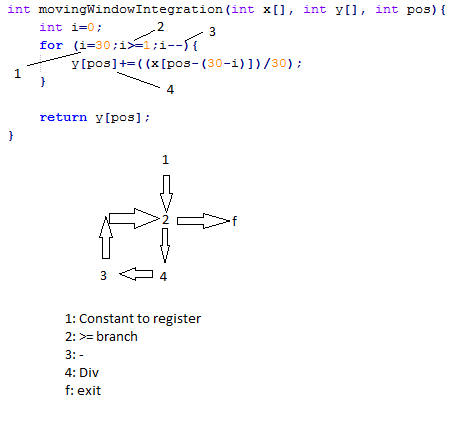
\includegraphics[width=0.75\textwidth]{C_to_assembly_diagram.png}
  \caption{A diagram depicting the translation from C to assembly code.}
\end{figure}

Once we had the block diagram, we proceeded with writing the actual assembly code itself. This code can be seen on figure 2 - seen below.

\begin{figure}[h!]
  \centering
    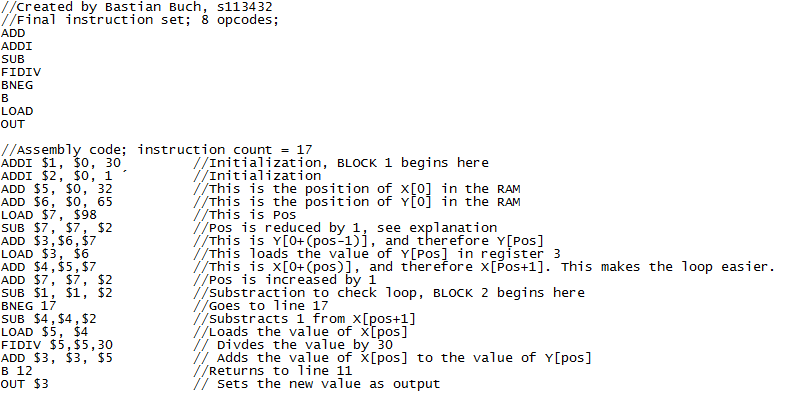
\includegraphics[width=0.75\textwidth]{screenshot_assembly.png}
  \caption{The assembly code.}
\end{figure}

We have implemented the assembler code with focus on minimizing the amount of instructions inside the "loop", as well as attempting to include as few operator codes as possible, generally attempting to use as few hardware resources as possible. This leads to some curious coding - substracting one from a 
register and adding one later, for example.\\
An explanation of our operator codes follow:\\
\begin{enumerate}
\item ADD, addition of two registers. First variable is the register saved to, second and third are the added registers.
\item ADDI, addition of register and integer. Same as ADD, with third register replaced by an int.
\item SUB, substraction of two registers. Syntax same as ADD, except substraction instead of addition.
\item FIDIV, division of a register with an integer. Same as ADDI, except the second register is divided with the integer.
\item BNEG, jump if negative. If the result of the previous calculation is negative, the assembler jumps to the line specified.
\item B, jump to. The assembler returns to the line specified with an integer.
\item LOAD, get external data. Data returns data to the first register, taken from the line of our RAM specified with the second register/integer
\item OUT, output external data. Returns the value of a register as output.
\end{enumerate}
\subsection{Implementation of the controller}
When implementing the controller, we would start out with building the datapath - that is, connecting the various components so they can actually calculate correctly, by initially creating the components that would be a part of the ADDI and the SUB/ADD assembly instructions. Once these datapaths were completed and connected, we would then start building the controller itself, whose job it would be to control the signals of the datapaths by defining the signals depending on the instruction set. The controller itself would be implemented as a separate datapath.
\subsection{Critical parts}
As we never got to implement the controller, we unfortunately could not evaluate the critical parts. However, had we managed to implement the controller, we would have evaluated the speed by the amount of clock cycles it would take to go through one data point on average. We would then look into what part of the program that requires the most time by loading in data from an external memory, and then use said data to evaluate the time - varying it throughout the testing to find out what takes the longest.\\
In regards to size, the simplest way to do so is to simply count the number of registries, adders, and multiplexers - along with their bit-width. When we were to then optimize it, we would look into which registries we might not need, and which we could reduce in width without compromising the integrity of the processor.\\
Finally, in regards to power consumption, there are generally three important terms to consider - Switching, which is power consumption because of active components; Short-circuit, which is when nMOS and pMOS transistors are on at the same time; and Static, which is power consumption because of inactive components. When we were to optimize, we would choose only to look at switching, as the amount of power needed goes up proportional with the activity - meaning that if the activity goes up a lot, the power consumption goes even higher.\\
One measures the amount of switching by looking at the amount of toggles there is per clock cycle - that is, the amount of bits switching from 0 to 1 or the other way around. Finding out just how many bits switch is quite easy in Gezel - we would just need to toggle on operation profiling, which is two commands. This would then show us the amount of evaluations and toggles, and through this tool, we would be able to see where we would need to optimize, and where we would be fine.\\

\section{Results}
The results and traces of our tests were intended to fully cover all possible errors in functionality.
For the ALU, this would mean testing all functions and checking their results to see if they were correct, for example, whereas the Multiplexer simply needs to demonstrate that the function picks the correct result.

Figure 3, 4, 5 and 6 are screenshots of the tests we have run on our basic modules.

\begin{figure}[h!]
  \centering
    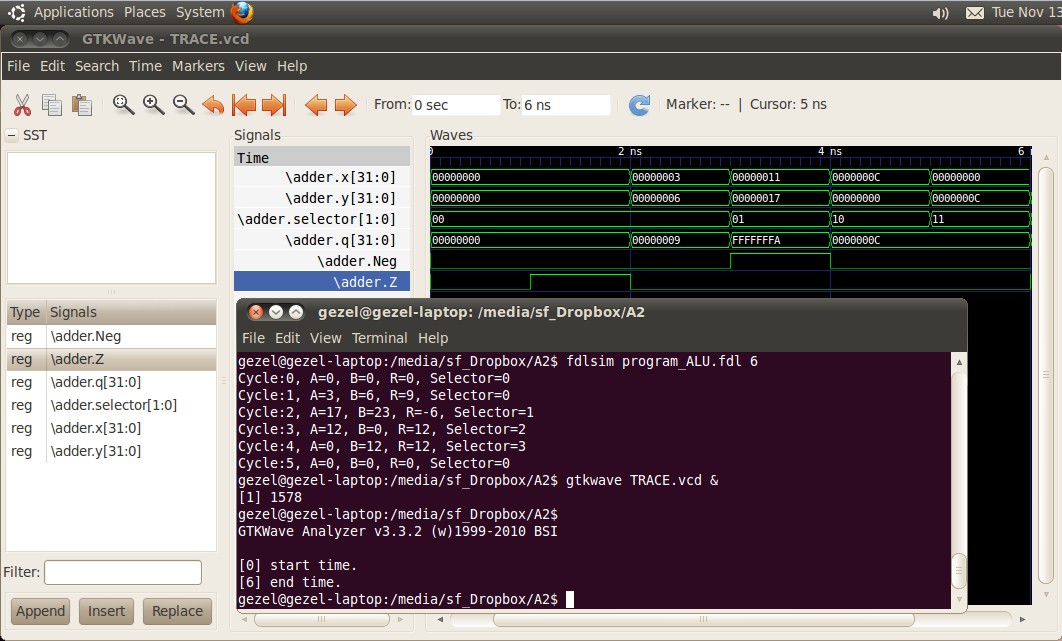
\includegraphics[width=0.75\textwidth]{results_ALU.png}
  \caption{The results of the ALU testbench.}
\end{figure}

\begin{figure}[h!]
  \centering
    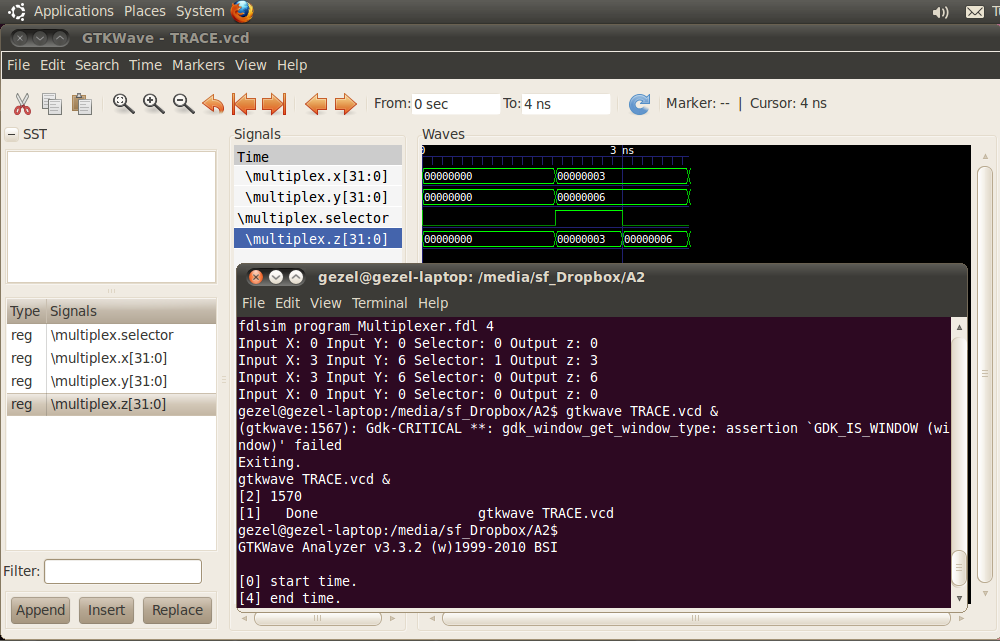
\includegraphics[width=0.75\textwidth]{results_Multiplexer.png}
  \caption{The results of the Multiplexer testbench.}
\end{figure}

\begin{figure}[h!]
  \centering
    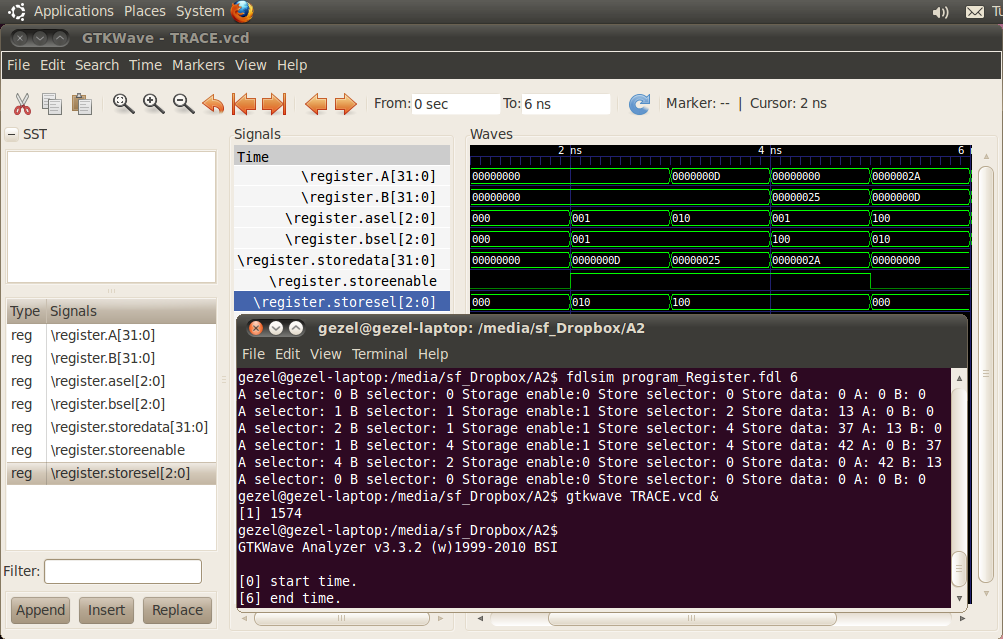
\includegraphics[width=0.75\textwidth]{results_Register.png}
  \caption{The results of the Register testbench}
\end{figure}

\begin{figure}[h!]
  \centering
    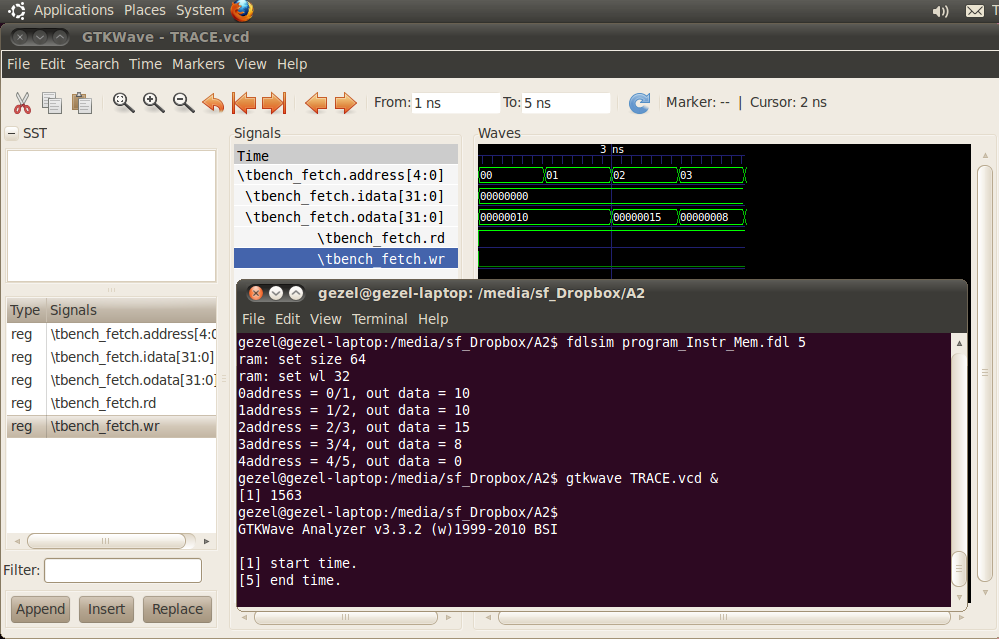
\includegraphics[width=0.75\textwidth]{results_Instr_Mem.png}
  \caption{The results of the RAM testbench}
\end{figure}

The screenshots consists of the gtkTrace result of all variables and their bit size minus one, as well as the test results from the terminal. If nothing is noted in the GTK next to the variable name, the variable is a single bit (1 or 0). \\
The ALU tests its functions after a zero cycle: \\
\begin{enumerate}
\item Addition
\item Substraction
\item Return X
\item Return Y
\end{enumerate}
The multiplexer tests its functions after a zero cycle:\\ 
\begin{enumerate}
\item Return X
\item Return Y
\end{enumerate}
The Register tests after a zero cycle:\\
\begin{enumerate}
\item Store in a register (register 2)
\item Read register 2 with A and store in register 4
\item Read register 4 as B and store again in register 4
\item Read register 4 with A and register 2 with B
\item Zero cycle (to counteract trace drop)
\end{enumerate}
The RAM block simply reads the lines from program.txt.\\
\\
As is quickly ascertained, the trace output the correct results from the variables.
It should be noted that Trace outputs the numbers in hexadecimal, and that the trace consistently does not recieve the results from the last clock cycle in the test. This has been compensated for by running an extra cycle, which is usually a test where all variables are zero.

\section{Conclusion}
	We did unfortunately not manage to implement the controller and thus, we could not analyse the performance of it either. However, we did create all the basic components of a processor, as well as the instruction set that the processor has to use for using the Moving Window Integration filter.
\newpage
\begin{thebibliography}{9}

\bibitem{lamport94}
  Michael Reibel Boesen, Linas Kaminskas, Karsten Juul Frederiksen and Dusan Vuckovich\\
  \emph{Assignment 2: The ECG processor}\\
  1st Edition\\
  2012.

\bibitem{Gezel Syntaks}
	Gezel Basic Syntaks pdf\\

\bibitem{Gezel user manual}
	\url{http://rijndael.ece.vt.edu/gezel2/manual.html} \\
	Date of use: 30/10-2012

\bibitem{Assembly language instruction set}
	\url{http://users.dickinson.edu/~braught/talksnpapers/ccscne01/KandS/instructions.html} \\
	Date of use: 10/11-2012
\end{thebibliography}
	
\newpage	
	\begin{Large}
		\textbf{Appendix}
	\end{Large}
	\appendix

\section{Who wrote what}
Jacob Gjerstrup, s113440 wrote: Introduction, Requirements, Analysis, Design, Implementation (50 percent), Abstract, Conclusion\\
Bastian Buch, s113432 wrote: Results, Instruction set (50 percent)\\
\\
For programming, a comment at each document has been made that shows whom programmed this particular part.
	
\section{Sourcecode}
\subsection{Basic Modules}
\subsubsection{Program Counter}
	\lstinputlisting{program_Counter.fdl}
	\newpage
\subsubsection{Adder}
	\lstinputlisting{program_Adder.fdl}
	\newpage
\subsubsection{ALU with flags}
	We have decided only to show the sourcecode of the extended ALU with flags, as it is identical to the standard ALU, except it holds a few more registers and calculations, which is used for calculating the flags.\\
	\lstinputlisting{program_ALU_flags.fdl}
\subsubsection{Multiplexer}
	\lstinputlisting{program_Multiplexer.fdl}
\subsubsection{Register}
	\lstinputlisting{program_Register.fdl}
\subsubsection{RAM}
	\lstinputlisting{program_Instr_Mem.fdl}
	\newpage
\subsubsection{Assembly Code}
	\begin{figure}[h!]
    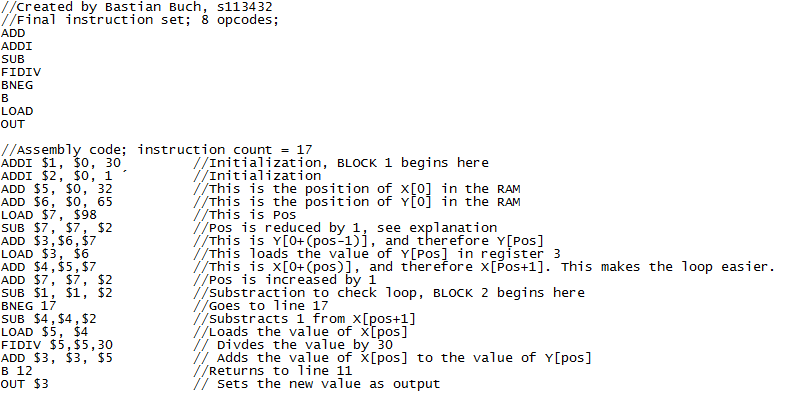
\includegraphics[width=0.75\textwidth]{screenshot_assembly.png}
\end{figure}
\end{document}